% !TEX root = sum1.tex
\section{Introduction}
Social distancing has been a proven concept to contain the spread of an infectious disease. As a general principle, social distancing can be implemented in various forms. The basic requirement of social distancing is the specification of a minimum physical distance between people in public areas. For example, the World Health Organization suggests social distancing by ``keep physical distance of at least 1 meter from others'' (https://www.who.int/emergencies/diseases/novel-coronavirus-2019/advice-for-public). In the US, the CDC refers to social distancing as ``keeping a safe space between yourself and other people who are not from your household.'' (https://stacks.cdc.gov/view/cdc/90522)

Note that under such a requirement, social distancing is actually applied with respect to groups of people. In Hong Kong, the government has adopted social distancing measures, in the recent Covid 19 pandemic, by limiting the size of groups in public gathering to two, four, and six people per group over time. Moreover, the Hong Kong government has also adopted the limit of the total number of people in a venue; for example, restaurants can operate at 50\% or 75\% of their normal seating capacity.


While the above practice of social distancing has been recognized for its primary function,  it is not clear how the entire economy will be affected. This is an important issue in the service sector where social distancing implies fewer clients and lower revenue. The situation is especially complicated under multiple social distancing measures, such as physical distance between groups, limit on the size of groups, and the occupancy rate of the venue. This naturally raises questions regarding the relationship of these measures, e.g., which is relatively more effective under different conditions, whether they compliment or contradict with each other, and more importantly, is it possible to align these measures so that they can be implemented coherently? 

We will address the above issues of social distancing in the context of seating arrangement in a venue, such as a cinema or a conference hall. The venue is equipped with seats of multiple rows.  People come in groups where each group of people will sit consecutively in one row. The social distancing requirement.


% Governments worldwide have been faced with the challenge of reducing the spread of Covid-19 while minimizing the economic impact. Social distancing has been widely implemented as the most effective non-pharmaceutical treatment to reduce the health effects of the virus. 
% This website records a timeline of Covid-19 and the relevant epidemic prevention measures\cite{Covid19Timeline}. For instance, in March 2020, the Hong Kong government implemented restrictive measures such as banning indoor and outdoor gatherings of more than four people, requiring restaurants to operate at half capacity. As the epidemic worsened, the government tightened measures by limiting public gatherings to two people per group in July 2020. As the epidemic subsided, the Hong Kong government gradually relaxed social distancing restrictions, allowing public group gatherings of up to four people in September 2020. In October 2020, pubs were allowed to serve up to four people per table, and restaurants could serve up to six people per table. Specifically, the Hong Kong government also implemented different measures in different venues \cite{Gov202209}. For example, the catering businesses will have different social distancing requirements depending on their mode of operation for dine-in services. They can operate at 50\%, 75\%, or 100\% of their normal seating capacity at any one time, with a maximum of 2, 2, or 4 people per table, respectively. Bars and pubs may open with a maximum of 6 persons per table and a total number of patrons capped at 75\% of their capacity. The restrictions on the number of persons allowed in premises such as cinemas, performance venues, museums, event premises, and religious premises will remain at 85\% of their capacity.


The measures implemented by the Hong Kong government primarily concentrate on restricting social distancing, group sizes and occupancy rates. However, implementing these policies in practice can pose challenges, particularly for fixed seating layouts with dynamic arrivals of people. In the original commercial case without social distancing requirements, customers did not need to sit together, so the focus was solely on total capacity. Under social distancing constraints, placing groups in row runs the risk of being unable to find matching demand, potentially leaving empty seats.

To avoid confusion, we clarify the distinction between `seat planning' and `seat assignment' which will be used in the following parts. In our context, the seat planning means the seat partition in the planning. The planning can be altered later when the planned seats don't match with the size of a coming group or when the seat planning is disrupted after assigning a coming group. In the seat assignment, for the coming group, when accepting it, we assign the seats to the group, and the seats will not be used by others in the future.

In order to adhere to social distancing guidelines, it is important to understand the process of generating seat planning based on known groups and how to assign seats to incoming groups. Additionally, it is of interest to explore how the social distancing constraints impact the sellers and the specific policies formulated by the government to address social distancing concerns.

We intend to shed light on the problem just described and to propose the practical dynamic seat assignment policy. In particular, we investigate the following questions. 

1. How can we model the seat planning problem given the social distancing restrictions? What kind of property does this problem have? How can we give a seat planning to accommodate the maximum people with stochastic demand?

2. How to use the property of seat planning problem to design the dynamic seat assignment policy? How good is the performance of this policy compared with other policies?

3. What kind of insights regarding the social distancing and occupancy rates can we obtain when implementing the dynamic seat assignment policy?

% In our study, we will focus on addressing this challenge in commercial premises, such as cinemas and music concert venues. We aim to provide a practical tool for venues to optimize seat assignments by proposing a seat assignment policy that takes into account social distancing requirements and the given seat layout. We strive to enable venues to implement social distancing measures effectively by offering a solution that provides specific seating arrangements.

To answer these questions, we construct the seat planning problem with deterministic and stochastic demand under social distancing requirement. For the deterministic situation, we have complete and accurate information about the demand for seating. We aim to provide a seat planning that maximizes the number of people accommodated. This situation is applicable in venues like churches or company meetings, where fixed seat layouts are available, and the goal is to assign seats to accommodate as many people as possible within the given layout. The seat planning obtained shows the utilization of as many seats as possible. Thus, we introduce the concept of full or largest pattern to indicate the seat partition of each row. For the seat planning that does not utilize all available seats, we propose to improve the seat planning by incorporating full or largest patterns.

For the stochastic situation, we have knowledge of the demand distribution before the actual demand is realized. We aim to generate a seat planning that maximizes the expected number of people accommodated. This approach is suitable for venues where seats have been pre-allocated to ensure compliance with social distancing rules. With the given demand scenarios, we develop the scenario-based stochastic programming to obtain the seat planning. To solve this problem efficiently, we apply the Benders decomposition technique. However, in some cases, solving the integer programming with Benders decomposition remains still computationally prohibitive. Thus, we can consider the LP relaxation then obtain a feasible seat planning by deterministic model. Based on that, we construct a seat planning composed of full or largest patterns to fully utilize all seats.

We mainly focus on addressing the dynamic seat assignment problem with a given set of seats in the context of social distancing. Solving the problem by dynamic programming can be prohibitive due to the curse of dimensionality, which arises when the problem involves a large number of variables or states. To mitigate this complexity, we begin by generating a seat planning in the stochastic situation. This seat planning acts as a foundation for the seat assignment. Then, we develop the dynamic seat assignment policy which guides the allocation of seats to the incoming groups sequentially. In the numerical result, our policy performs well compared with other policies. 
We use $\tilde{T}$ to denote the gap point, which refers to the first time period at which, on average, the number of people accepted without social distancing is not less than that accepted with social distancing plus one. By sampling many probability combinations, the results show that $\tilde{T}$ and the corresponding occupancy rate, $\beta(\tilde{T})$, can be estimated with $\gamma$, the expected number of people per period. Different $\gamma$ corresponds to different $\tilde{T}$. When the total number of periods, $T$, is less than $\tilde{T}$, we tend to accept all incoming groups. In this case, there is no difference whether to implement the social distancing restriction. When $T$ is larger, there will be more groups rejected when implementing the social distancing requirement. The government can consider the potential losses when making policies regarding group size and occupancy rate. Similarly, the seller can implement corresponding measures to adhere to these requirements.

% Regarding the seat assignment with social distancing constraint, we consider the dynamic demand based on the seat planning. For the dynamic situation, the decision to accept or reject a group is made for each incoming group. This situation is commonly encountered in venues such as cinemas or music concerts, where decisions can be made on a group-by-group basis. The goal is to make timely decisions regarding seat assignments, considering factors such as available seating capacity, social distancing requirements and the specific size of each group.

% The following figures illustrate the seat planning and seat assignment. 

% \begin{figure}[htbp]
%     \centering
%     \begin{minipage}[t]{0.48\textwidth}
%     \centering
%     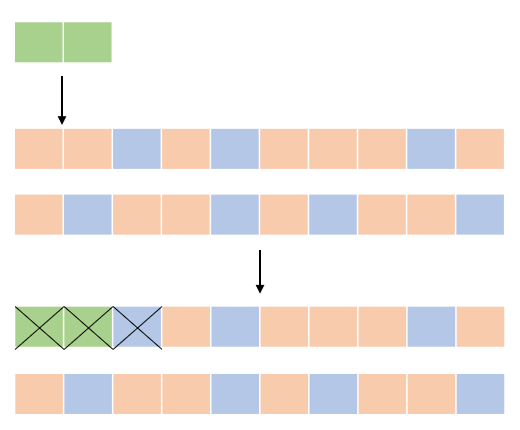
\includegraphics[width=5cm]{./Figures/seat_assign1.png}
%     \caption{Assign The Group in Row 1}
%     \end{minipage}
%     \begin{minipage}[t]{0.48\textwidth}
%     \centering
%     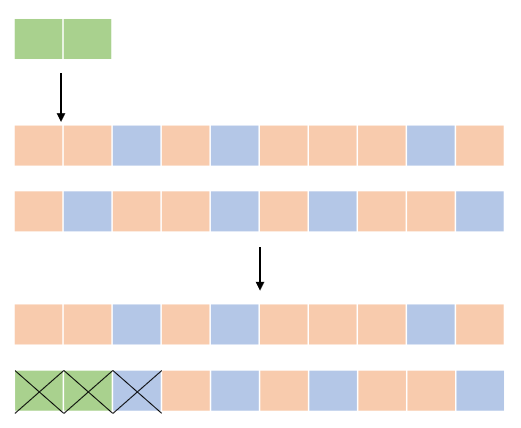
\includegraphics[width=5cm]{./Figures/seat_assign2.png}
%     \caption{Assign The Group in Row 2}
%     \end{minipage}
% \end{figure}


Our main contributions in this paper are summarized as follows. First, this study presents the first attempt to consider the arrangement of seat assignments with social distancing under dynamic arrivals. While many studies in the literature highlight the importance of social distancing in controlling the spread of the virus, they often focus too much on the model and do not provide much insight into the operational significance behind social distancing \cite{barry2021optimal, fischetti2021safe}. Recent studies have explored the effects of social distancing on health and economics, mainly in the context of aircraft \cite{salari2020social, ghorbani2020model, salari2022social}. Our study provides a new perspective to help the government adopt a mechanism for setting seat assignments to implement social distancing during pandemic.

Second, we establish a deterministic model to analyze the effects of social distancing when the demand is known. Due to the medium size of the problem, we can solve the IP model directly. We then develop the scenario-based stochastic programming by considering the stochastic demands of different group types. By using Benders decomposition methods, we can obtain the seat planning quickly. 

Third, to address the problem in the dynamic situation, we first obtain a feasible seat planning from scenario-based stochastic programming. We then make a decision for each incoming group based on our dynamic seat assignment policy, either accepting or rejecting the group. Our results demonstrate a significant improvement over the traditional control policies and provide the insights on the implementation of social distancing.

% Our results demonstrate the effectiveness of our approach in balancing social distancing requirements with revenue generation, providing valuable insights for policymakers and venue managers. Specifically, our proposed approach can help cinemas, concert venues, and other public spaces optimize seat assignments while ensuring the safety of patrons. It provides a practical tool for venues to implement social distancing measures in a flexible and efficient manner, adapting to changes in demand and maximizing revenue generation while maintaining social distancing measures.

% With this new .., we illustrate how to assign the seats by the govenment/stakeholder to balance health and economic issues. In addition, we also provide managerial guidance for the government on how to publish the related policy to make the tradeoff between economic maintenance and risk management.

The rest of this paper is structured as follows. The following section reviews relevant literature. We describe the motivating problem in Section 3. In Section 4, we establish the stochastic model,analyze its properties and obtain the seat planning. Section 5 demonstrates the dynamic seat assignment policy to assign the seats for incoming groups. Section 6 gives the numerical results and the insights of implementing social distancing. The conclusions are shown in Section 7.
\newpage
